%=== CHAPTER FOUR (4) ===
%=== Test and Experiments ===

\chapter{Experiments}
\begin{spacing}{1.5}
\setlength{\parskip}{0.3in}
\section{Dataset}
To the best of the authors' knowledge, there is currently no dataset for studies of skin blemish modification and fading. Therefore, a self-collected dataset is adopted for research, development, and testing. The images within the dataset were acquired by two clinical imaging systems (Visia CR4 and OLE, both developed by Canfield Scientific). They were cross-polarized and color-calibrated and had a minimum resolution of $3700 \times 5600$. The dataset consists of 223 subjects within the age range of 18 to 45 years, encompassing multi-ethnic consumers with skin tones ranging from dark to light, quantitatively assessed using the Individual Typology Angle (ITA), visualized in Figure \ref{fig:ita}. The ITA for each subject is calculated using the formula:
\begin{equation}
\text{ITA} = \arctan\left(\frac{L* - 50}{b*}\right) \times \frac{180}{\pi},
\end{equation}
where $L*$ and $b*$ are coordinates from the CIE-LAB color space representing the lightness and the chromaticity on the yellow/blue axis, respectively. This measure provides a valuable tool for analyzing skin tone diversity in the dataset. The collection period lasted for a duration of up to 3 months during the Summer season with a time step of one week. The summary of the dataset is shown in Table \ref{tbl:dataset_summary}. In the simulation, images of Week 0 are input and the parameters of the obtained model are adjusted to simulate the change of the blemishes in the following weeks. As shown in Figure\ref{fig:forward}, the input is labelled as \textit{Week 0} and the images for the next few weeks as \textit{+n W}.

\begin{table}[t!]
    \caption{Summary of Dataset Statistics}
    \resizebox{\columnwidth}{!}{%
    \begin{tabular}{lrlrlr}
        \toprule
        \multicolumn{2}{c}{\textbf{ITA Score}} & \multicolumn{2}{c}{\textbf{Ethnicity}} & \multicolumn{2}{c}{\textbf{Skin Tone Classification}} \\
        \midrule
        \midrule
        Total Subjects        & 223   & African       & 126 & Dark         & 76 \\
        ITA Mean              & 2.58  & Caucasian     & 98  & Brown          & 132  \\
        ITA Variance          & 851.90 & Indian       & 108 & Tan           & 152 \\
                              &       & Latino        & 114 & Intermediate  & 62 \\
                              &       &               &     & Light         & 8   \\
        \bottomrule
    \end{tabular}
    }
    \label{tbl:dataset_summary}
\end{table}
\begin{figure}[t!]
    \centering
    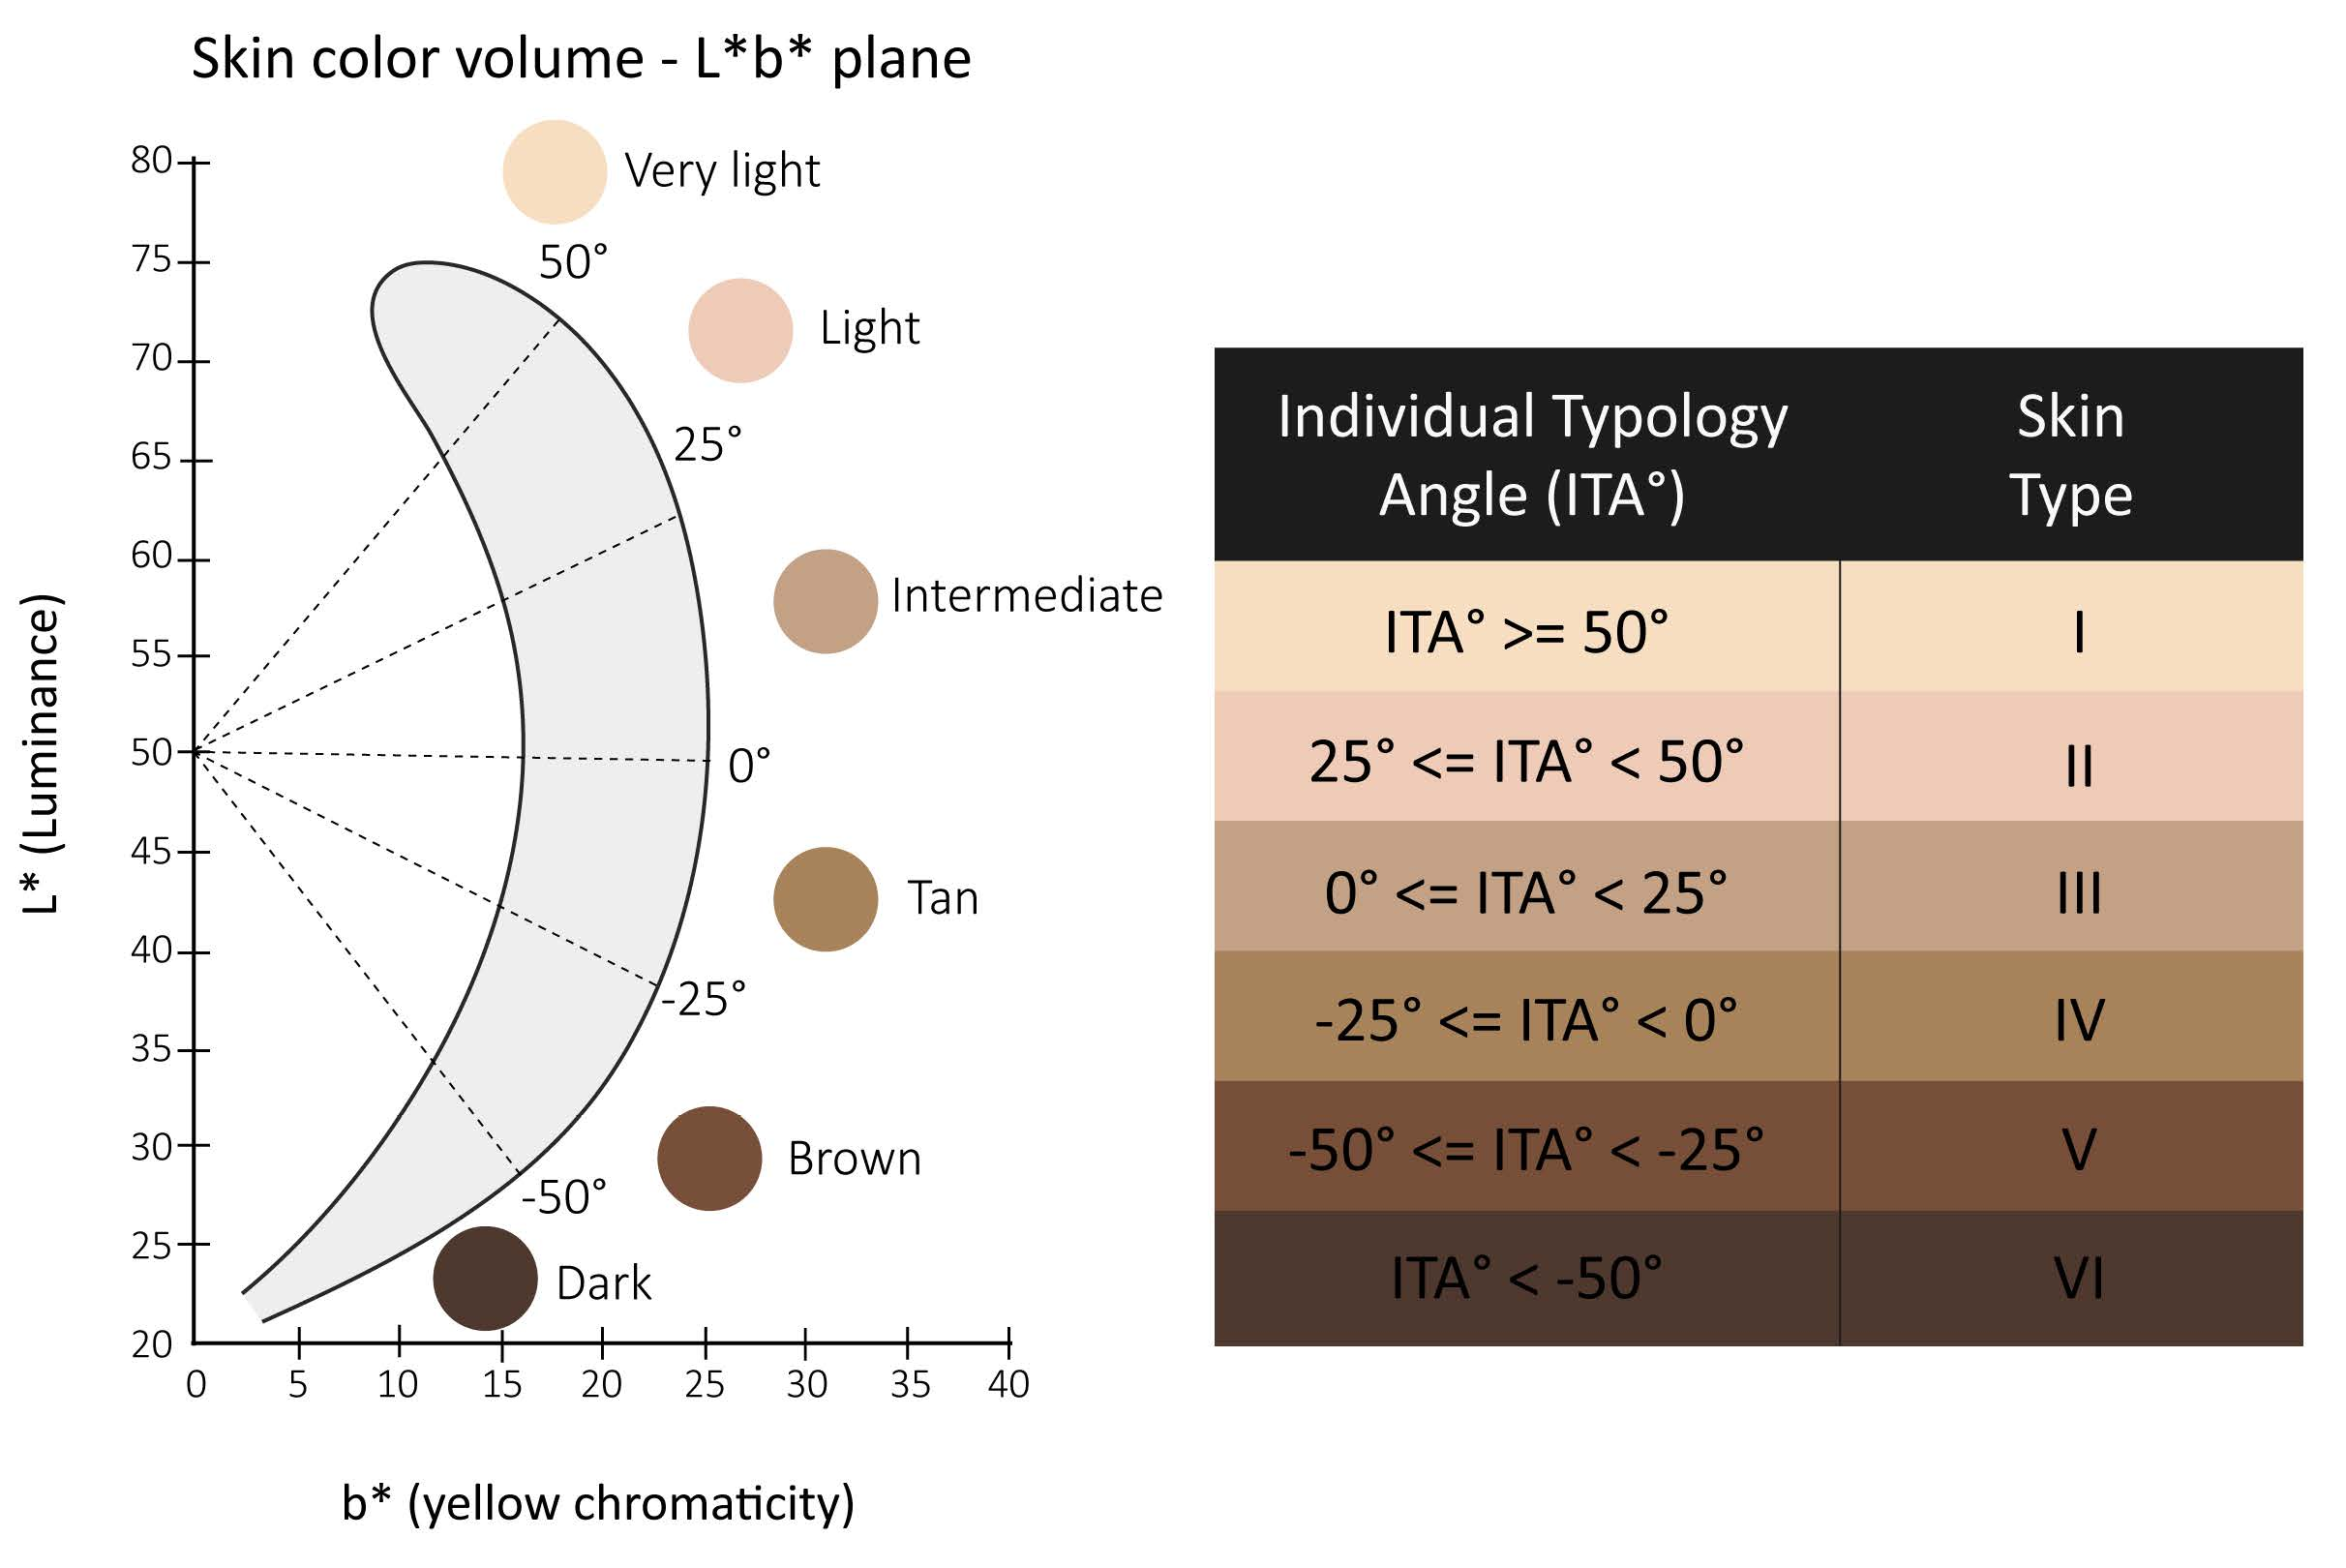
\includegraphics[width=0.97\columnwidth]{Chapter4/ITA.jpg}
    \caption{Visualisation of ITA classification threshold within the L* and b* color space, used for determining skin tone categories. The left side shows the skin color volume on the L*-b* plane with indicative angles for various skin tones, while the right side presents specific ITA ranges with corresponding skin rone classifications from I (very light) to VI (dark). Our dataset encompasses a diverse spectrum of skin tones, including categories from dark (Skin Type VI) to light (Skin Type II). Image taken from \cite{krishnapriyaAnalysisManualAutomated2022a}.}
    \label{fig:ita}
\end{figure}

\section{Experiment Setup}
In this study, extensive blemish change simulation experiments are carried out to evaluate the proposed algorithm's effectiveness. Each blemishes is fitted with 3 Gaussian functions summation and $\sigma=10$ is set for the skin texture layer separation filter. The focus is mainly on the relative concentration changes of the blemishes, and a series of simulations are conducted based on tuning the concentration parameter after successfully fitting blemishes.

Inpainting mode of \textbf{Stable Diffusion}(SD)\cite{rombach2021highresolution} and \textbf{Adobe Photoshop}(PS)'s inpainting tool\cite{adobephotoshop} are selected for comparison as baseline models, as shown in Figure \ref{fig:ps_sd}. The former, a top-performing deep learning model, represents the "latent space editing" method discussed. For the SD method, the inpainting mode is used and the text prompt is set as \texttt{skin patch, human face skin, high definition, best quality}, as shown in Figure \ref{fig:sd}. Each test is performed with 50 iterations of sampling using the \texttt{DPM++SDE Karras} sampler, with the random seed fixed to 42. The denoising ratio is adjusted to increase the difference between the generated image and the original so that the intensity of blemish removal is controlled. 

For the PS method, a common image editing software, represents the "pixel space editing" method. Here, the inpainting tool is utilized, selecting and removing blemishes on the original image with \textit{Content-Aware} mode, as shown in Figure \ref{fig:ps}. The modified image is then combined with the original image through Alpha blending. And the degree of blemish removal is adjusted by altering blending opacity.

\begin{figure}[t!]
    \centering
    \begin{subfigure}{.97\textwidth}
        \centering
        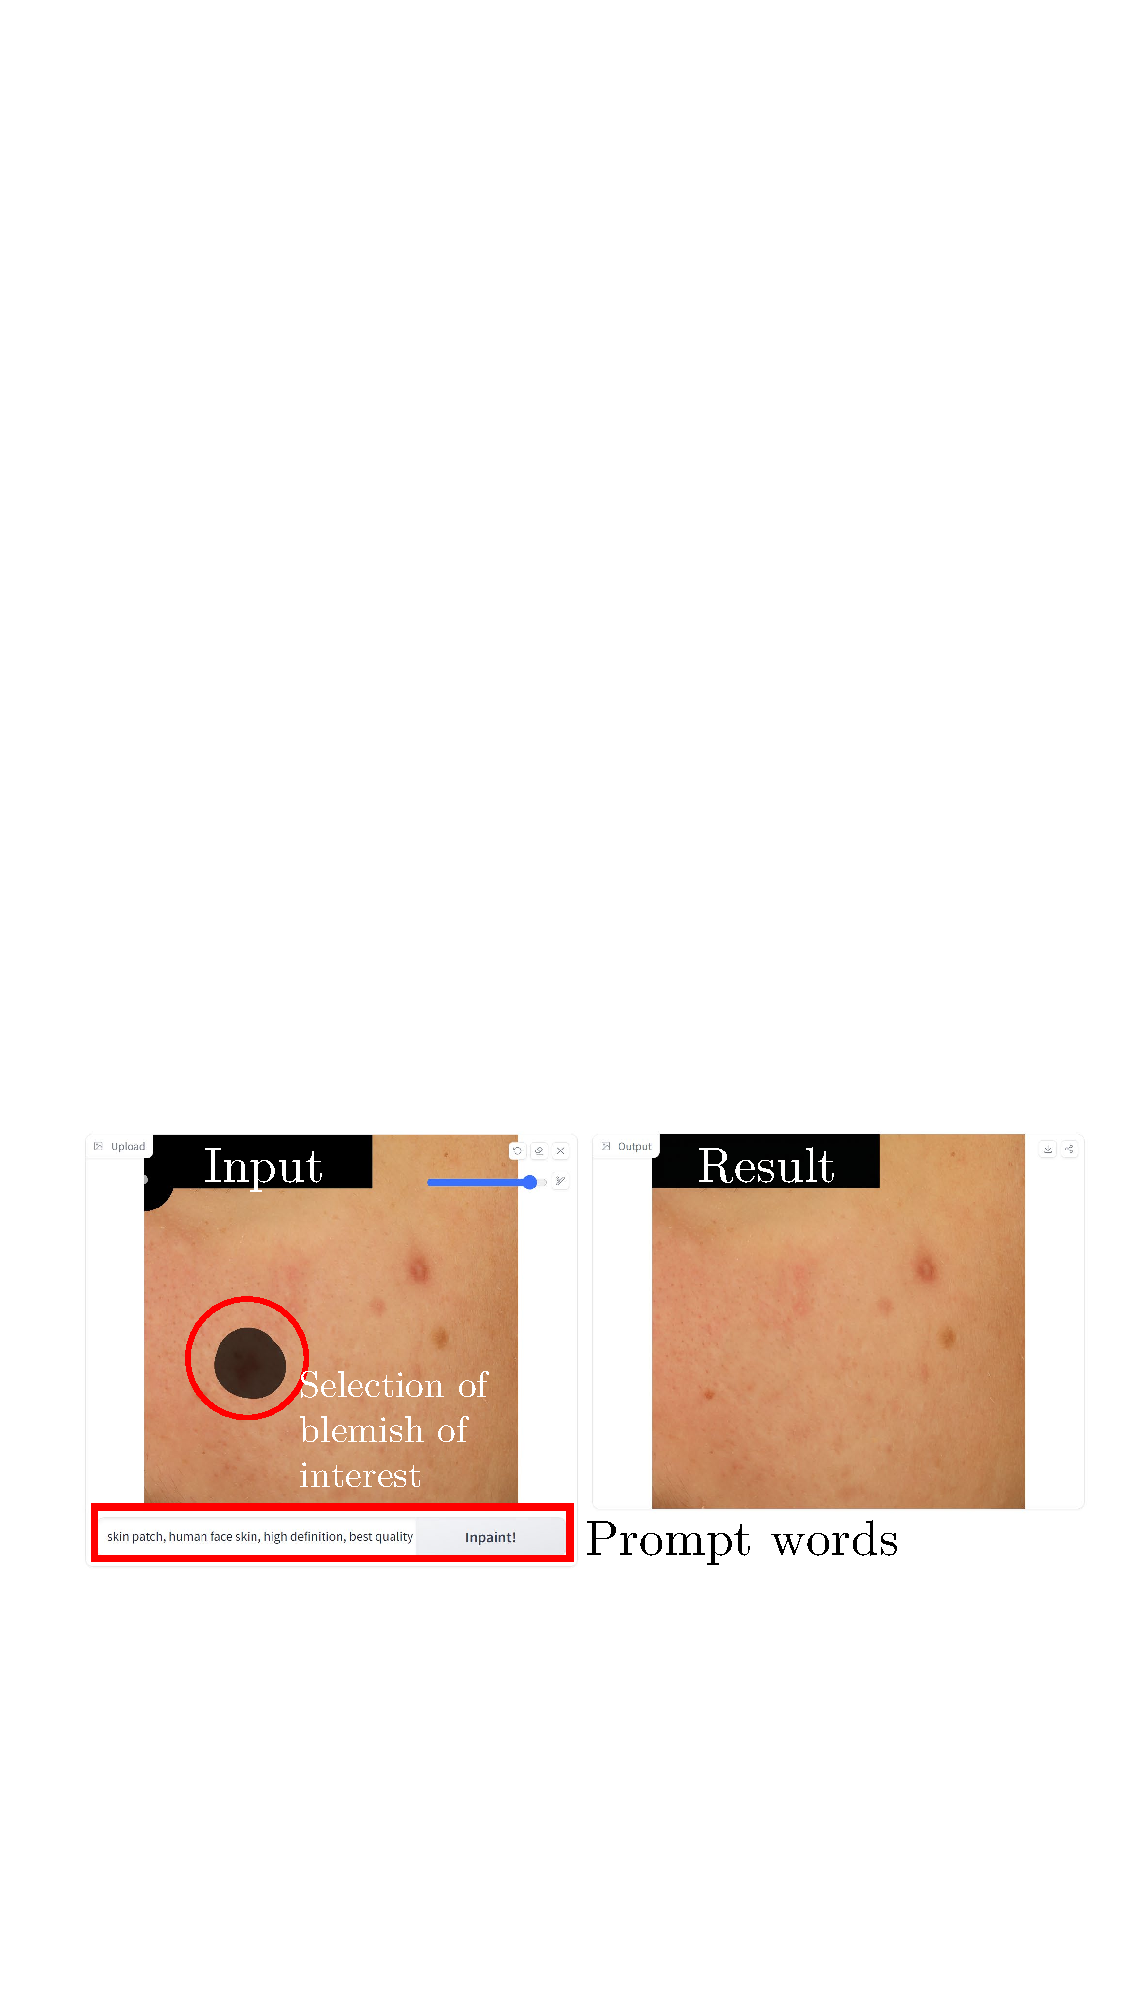
\includegraphics[width=0.97\columnwidth]{Chapter4/sd_ui.pdf}
        \caption{Stable Diffusion (SD) inpainting mode}
        \label{fig:sd}
    \end{subfigure}\hfill
    \begin{subfigure}{.97\textwidth}
        \centering
        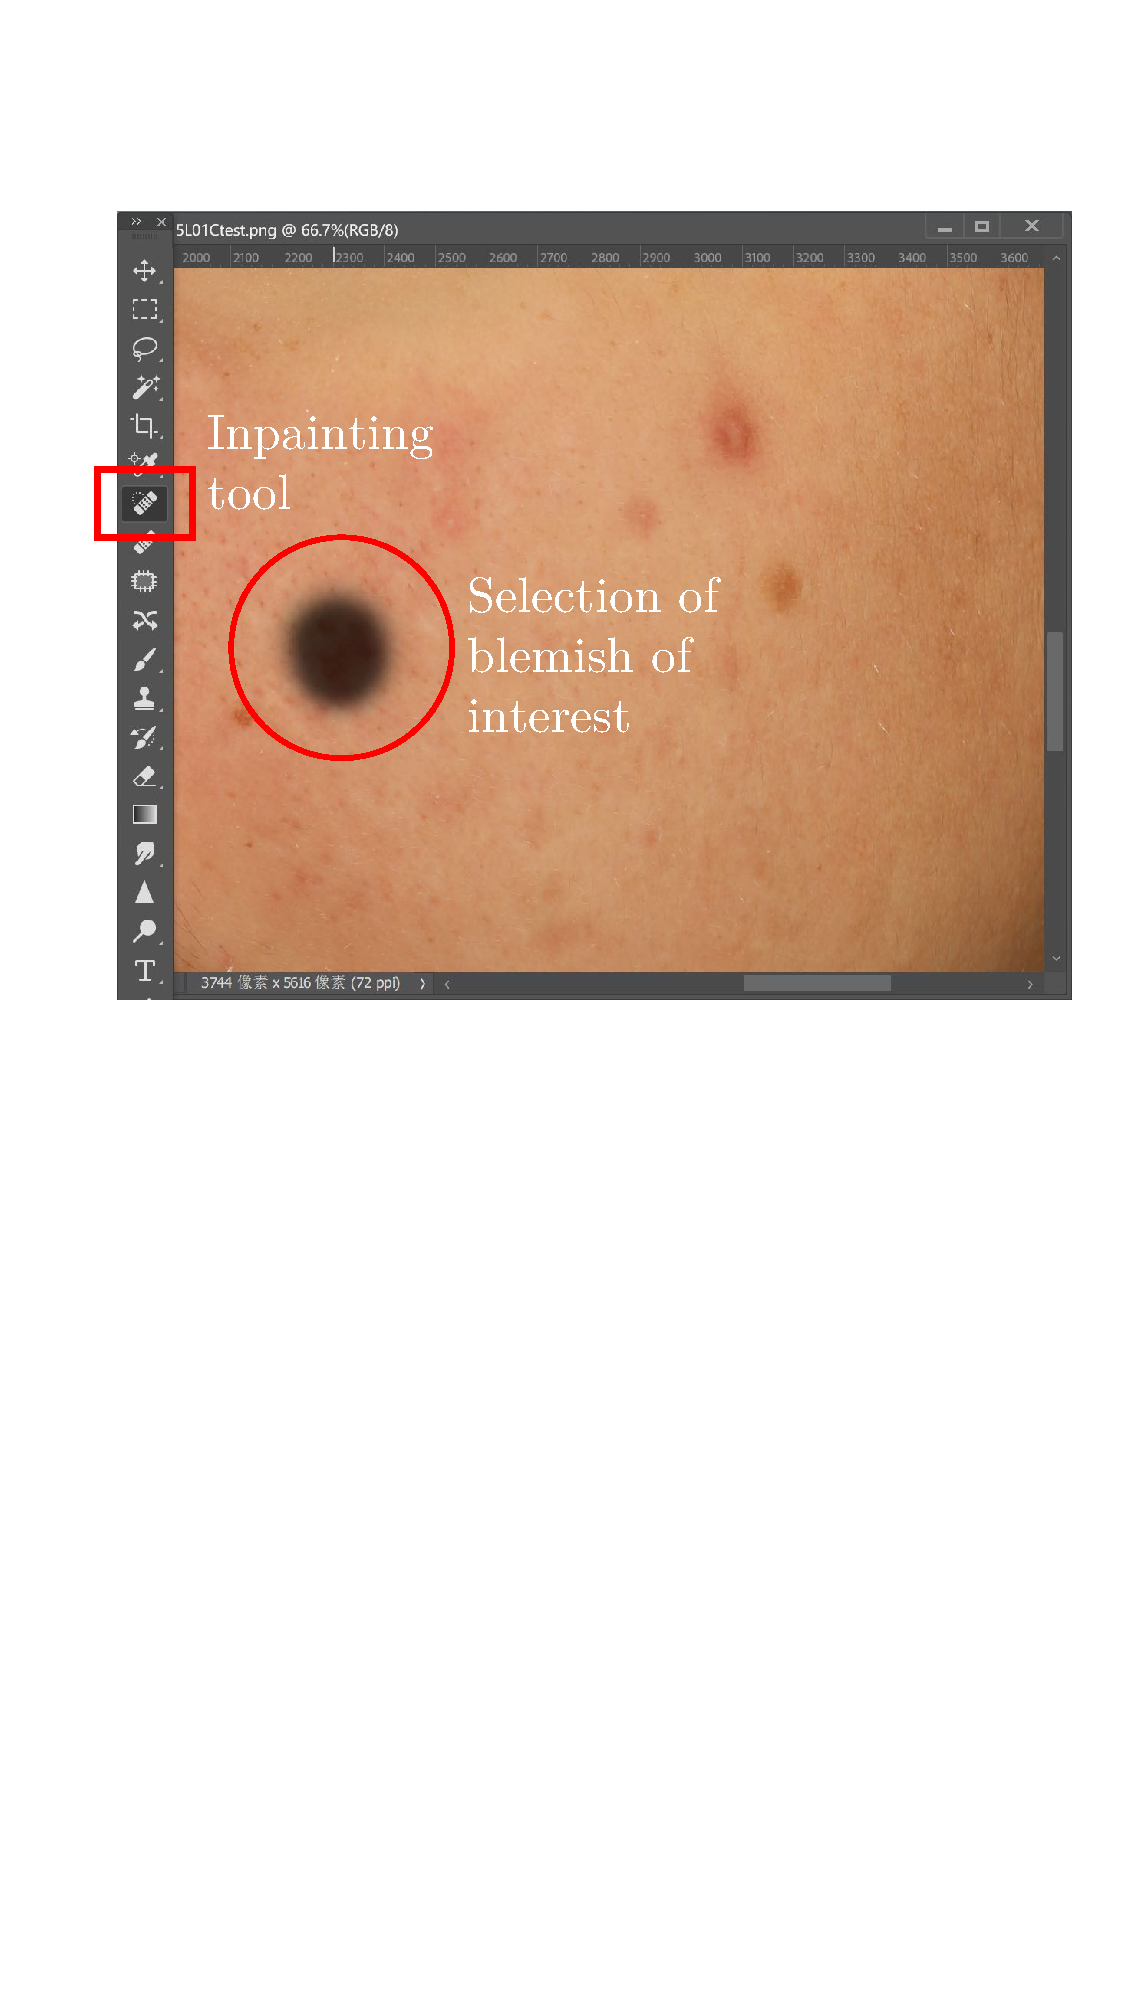
\includegraphics[width=0.97\columnwidth]{Chapter4/ps_ui.pdf}
        \caption{Adobe Photoshop (PS) inpainting tool}
        \label{fig:ps}
        % \label{fig:gui1}
    \end{subfigure}
    \caption{Example of a baseline models. Widely available and easily reproducible baseline methods are selected for comparison. Specifically, Adobe Photoshop(PS) is chosen For \textit{pixel space} editing methods, which is the most commonly used image editing and retouching software. For \textit{latent space} editing methods, Stable Diffusion(SD), recognised for its high-quality generation, is selected.}
    \label{fig:ps_sd}
\end{figure}

\subsection{Objective Evaluation}
To objectively evaluate image modifications, the Fréchet Inception Distance (FID) is applied. FID is a common tool for assessing GANs and similar image-generating models. It uses the Inception V3\cite{DBLP:conf/cvpr/SzegedyVISW16} model to derive the mean and covariance matrix of feature vectors from both authentic and generated image collections. Then, it calculates the Fréchet distance between these statistical groups. This distance gauges the variation between two multi-dimensional Gaussian distributions. Generated images resembling real images more closely have lower FID scores, while higher scores show a bigger divergence. Formally, the FID score is denoted as:
\begin{equation}
    \text{FID} = \|\mu_r - \mu_g\|^2 + \text{Tr}(\Sigma_r + \Sigma_g - 2(\Sigma_r\Sigma_g)^{1/2}),
\end{equation}
where $\mu_r, \mu_g$ represent the mean feature vectors of the real and generated/modified images, respectively. $\Sigma_r, \Sigma_g$ are the covariance matrices of the real and generated/modified images, respectively. And $\text{Tr}(\cdot)$ is the trace of a matrix, which is the sum of the diagonal elements.
% TODO
\subsection{Subjective Evaluation}
To subjectively evaluate the performance of the proposed facial skin blemish simulation algorithm, a visual perception study is conducted. The aim is to comprehensively evaluate whether the proposed algorithm could produce authentic and believable blemish changes and to analyse whether there are biases in certain attributes of the skin, such as skin color or age. A group of 500 panellists join this study, whose age groups are divided into three categories: 19-25; 26-34; and 35-45, covering various ethnicities including Caucasians, African-Americans, Asians, Hispanics, and others, as shown in Figure \ref{fig:metadata}.
\begin{figure}[t!]
    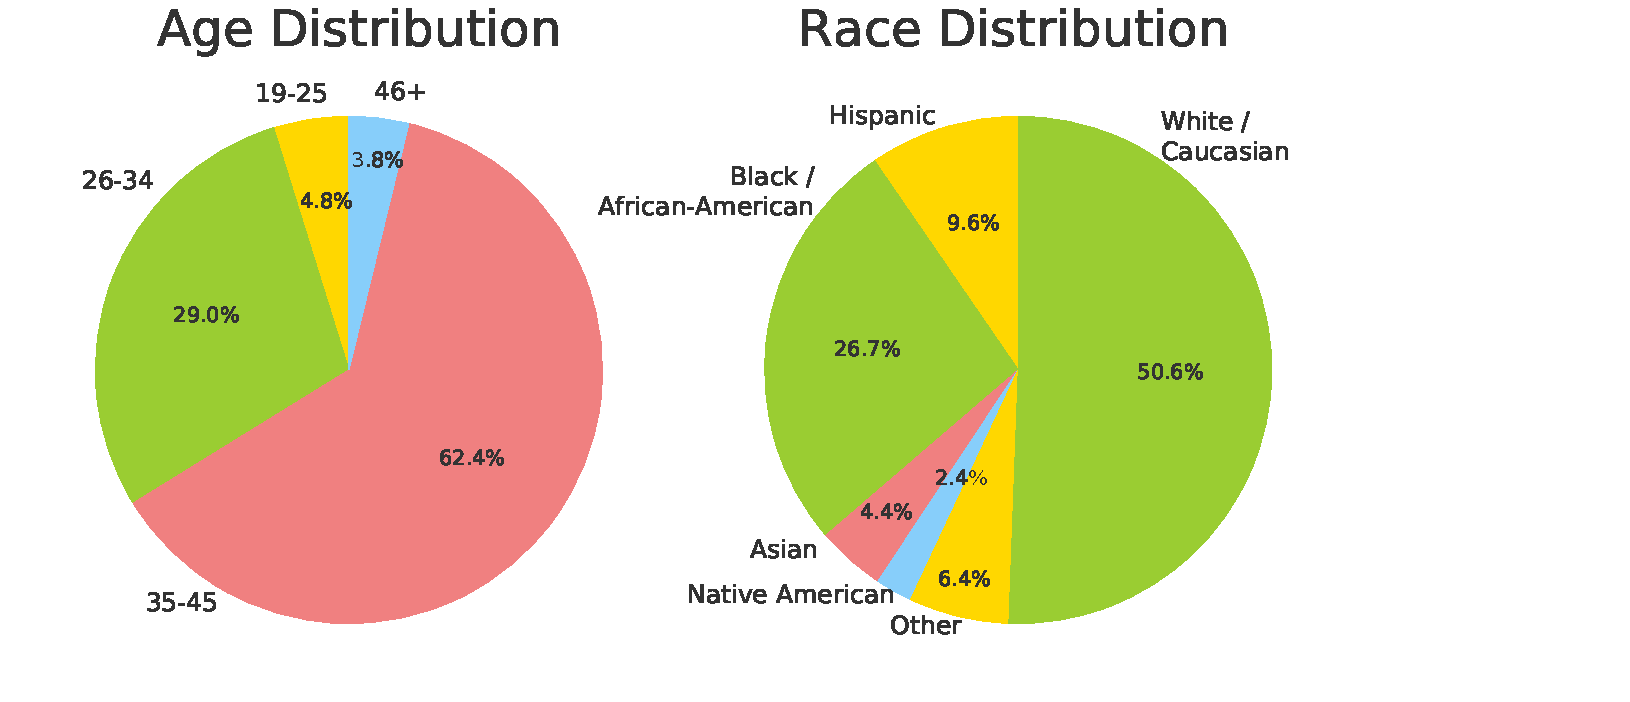
\includegraphics[width=0.95\columnwidth]{Chapter4/metadata.pdf}
    \caption{Metadata of panellists. The test population covers people from 19 to 45 years old, multiple races, and multiple skin tones}
    \label{fig:metadata}
\end{figure} 
\begin{figure}[t!]
    \centering
    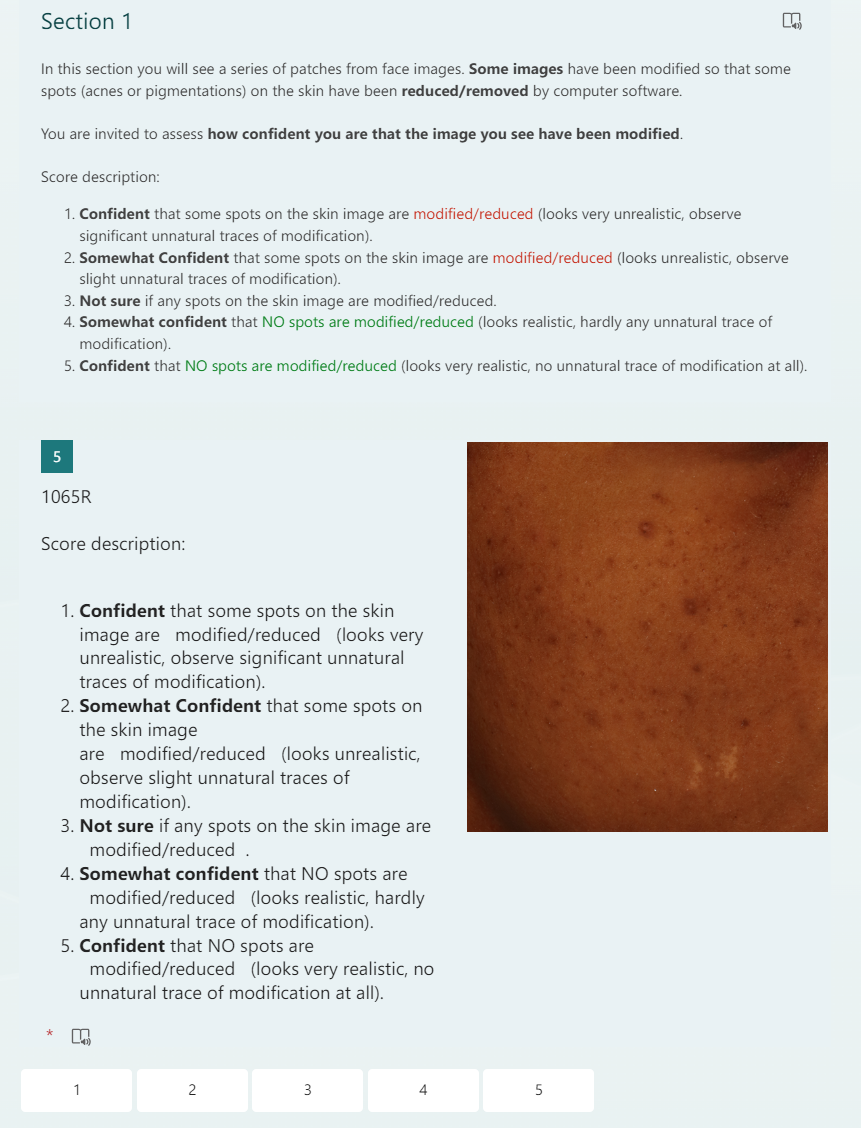
\includegraphics[width=0.9\columnwidth]{Chapter4/sample_form1.png}
    \caption{Examples of questions in the questionnaire. We designed 48 such questions, with 24 featuring modified images. For each panellist, we randomly select 10 questions from the question bank.}
    \label{fig:sample_form}
\end{figure}
In the survey, the question asked is \textit{you will see a series of patches from face images. Some images have been modified so that some spots (acnes or pigmentations) on the skin have been reduced/removed by computer software. You are invited to assess how confident you are that the image you see have been modified.} The answer options are set as:
\begin{itemize}
    \item Confident that some spots on the skin image are modified/reduced (looks very unrealistic, observe significant unnatural traces of modification). (-2)
    \item Somewhat Confident that some spots on the skin image are modified/reduced (looks unrealistic, observe slight unnatural traces of modification). (-1)
    \item Not sure if any spots on the skin image are modified/reduced. (0)
    \item Somewhat confident that NO spots are modified/reduced (looks realistic, hardly any unnatural trace of modification). (+1)
    \item Confident that NO spots are modified/reduced (looks very realistic, no unnatural trace of modification at all). (+2)
\end{itemize}

In the survey, 48 images (24 simulated through the proposed algorithm and 24 unaltered images) are shown to the panellists one image at a time. When the score ranges from 0 to +2, the respondents are considered to be affirming the image as "real" rather than modified. A sample question in the survey is shown as Figure \ref{fig:sample_form}.
%=== END OF CHAPTER FOUR ===
\end{spacing}
\newpage
